\section{Who provides reversion? An equilibrium}\label{sec:equil}

Proposition~\ref{prop:sum} says that transient risk is governed by one ratio, $S=\tilde\kappa/(m-q\tilde\kappa)$. Its ingredients are chosen by market participants: dealers decide how hard to lean against price displacements, which sets reversion $m$, and momentum traders decide how strongly to chase them, which sets $q$. This section asks whether those choices are efficient.

\subsection{Setup}
There are $N$ dealers. Dealer $i$ supplies reversion intensity $s_i\ge0$ by absorbing order flow against the displacement, so $m=m_0+\sum_is_i$, where $m_0$ is reversion supplied by other means. Leaning earns a spread $v$ per unit of intensity at quadratic inventory cost, so the private value is $vs_i-\tfrac c2s_i^2$. By Theorem~\ref{thm:guard} the worst-case transient loss of a position of size $Q$ facing flow shocks bounded by $U$ is $QU\,S$, so we take aggregate expected tail loss to be $\Lambda S(m,q)$ with $\Lambda>0$. Dealers bear a share $\theta<N$ of it, so each bears $\theta/N$; leveraged users and their counterparties bear the rest. Momentum traders choose aggregate intensity $q$ with private value $bq-\tfrac e2q^2$ and bear none of the tail loss. Long-run impact $\tilde\kappa$ is taken as given.

\subsection{Results}

\begin{proposition}[Equilibrium transient risk]\label{prop:equil}
Let $g(m)\equiv-\partial S/\partial m=\tilde\kappa/(m-q\tilde\kappa)^2$.
\begin{enumerate}[label=(\roman*)]
\item \emph{Under-provision of reversion.} The symmetric Nash equilibrium solves $m-m_0=N v/c+\theta\Lambda g(m)/c$, the planner's optimum solves $m-m_0=N v/c+N\Lambda g(m)/c$, and $m^{\rm eq}<m^{\rm SP}$, so $S^{\rm eq}>S^{\rm SP}$.
\item \emph{Fewer dealers, more risk.} $\partial m^{\rm eq}/\partial N=(v/c)/(1-\theta\Lambda g'(m)/c)>0$, so equilibrium reversion rises and $S^{\rm eq}$ falls with the number of dealers.
\item \emph{Over-provision of momentum.} Momentum traders choose $q=b/e$; the planner chooses $q^{\rm SP}<b/e$, solving $b-eq=\Lambda\tilde\kappa^2/(m-q\tilde\kappa)^2$.
\item \emph{The corrective price is identified.} The first best for reversion is implemented by a rebate per unit of reversion
\[
\tau^*=\Bigl(1-\frac\theta N\Bigr)\Lambda\,g(m)=\Bigl(1-\frac\theta N\Bigr)\Lambda\,\frac{S^2}{\tilde\kappa},
\]
which depends on the market only through $S$ and $\tilde\kappa$.
\end{enumerate}
\end{proposition}

\begin{proof}
(i) Dealer $i$'s first-order condition is $v-cs_i+(\theta/N)\Lambda g(m)=0$; the planner's is $v-cs+\Lambda g(m)=0$. Summing over dealers gives the two fixed-point equations. The right-hand sides are decreasing in $m$ because $g$ is decreasing on $m>q\tilde\kappa$, and the planner's lies above the dealers' for every $m$ when $\theta<N$, so its crossing with the line $m-m_0$ lies to the right. (ii) follows by implicit differentiation, since $g'<0$. (iii) $\partial S/\partial q=\tilde\kappa^2/(m-q\tilde\kappa)^2>0$ is the marginal external cost of momentum that traders ignore. (iv) The rebate closes the wedge between the two first-order conditions, and $g=S^2/\tilde\kappa$ by Proposition~\ref{prop:sum}.
\end{proof}

At $v=0.002$, $c=0.5$, $\theta=0.3$, $\Lambda=10^{-4}$, $m_0=0.005$, $q=0.02$ and $\tilde\kappa=1$, equilibrium $S$ falls from 27.9 with one dealer to 6.8 with forty, and the planner's $S$ is 1.5--2.7 times lower throughout; the rebate computed from $S$ alone coincides with the first-order wedge to machine precision. With $m=0.03$, $b=0.3$ and $e=20$, momentum traders choose $q=0.015$ against a planner's $0.0062$.

\paragraph{Interpretation.} Reversion is a public good: each dealer who leans against a displacement lowers the tail exposure of every leveraged position in the market but is paid only for his own fills. Momentum is the mirror image. Part (iv) closes the loop with the guard: the policy price of the externality is a function of the same summed response that the guard bounds, and Propositions~\ref{prop:invariance} and~\ref{prop:bridge} show that this quantity is identified from public data without identifying the traders. A venue that rebates reversion in proportion to $S^2/\tilde\kappa$, or a supervisor that sets pre-trade limits by $S$, prices the externality with an observable.

\paragraph{What the data say about the model's predictions.} Part (ii) predicts that books with fewer dealers have higher $S$ because they supply less reversion. Depth is the closest proxy we observe for the number of liquidity providers. Across the three liquidity terciles of the 30 Binance perpetuals on training days, the summed response per dollar of flow rises steeply as depth falls (median $2{,}797$, $26{,}603$ and $39{,}329$ basis points per \$1M in the thick, mid and thin terciles; Spearman correlation with log depth $-0.94$), as (ii) predicts. The channel is not the one the model names, however: the unit-free gain multiple $S/|h_0|=1/(m-q\tilde\kappa)$, which isolates reversion net of momentum, is the same in all three terciles (medians $46.4$, $47.3$ and $46.9$; Spearman $-0.11$). Thinner books carry more cumulative risk because their impact $\tilde\kappa$ is larger, not because they revert more slowly. These comparisons were made after the fact (Part 13, \texttt{R2}), and depth is an imperfect proxy for dealer count, so a direct test needs data on liquidity-provider identities. The model's second prediction, that the dynamic balance forecasts tail losses where reversion is close to $q\tilde\kappa$, is what Section~\ref{sec:thin} tests.

\section{Information limits, safety certification, and the value of disclosure}\label{sec:flagship}

The guard of Section~\ref{sec:guard} requires the cumulative impulse response, whereas the companion paper establishes sharp limits on what finite market histories reveal about hidden adaptive cohorts. We now answer the unified question connecting the two papers: when the adaptive systems operating inside a market are only partially observed, what information is sufficient to certify safe trading decisions, what does that information cost, and how much financially valuable trading must be sacrificed when information is insufficient?

\subsection{An exact two-market ambiguity witness and information--safety impossibility}
Consider the positive-memory cohort economy $x_{t+1}=ax_t+\sum_{i=1}^K y_{i,t}+u_t$, $y_{i,t+1}=(1-\eta_i)y_{i,t}+\eta_i q_i x_t$ with $a=2/5=0.40$ and zero initial memory states. Table~\ref{tab:witness} and Figure~\ref{fig:flagship1} construct two asymptotically stable markets in exact rational arithmetic (test \texttt{T01}).

\begin{table}[t]\centering\small
\begin{threeparttable}
\caption{Two-market ambiguity witness (\texttt{T01})}\label{tab:witness}
\setlength{\tabcolsep}{6pt}
\begin{tabular}{lcc}
\toprule
Quantity & Market A ($K=1$) & Market B ($K=2$)\\
\midrule
Memory rates $\eta_i$ & $1/2=0.50$ & $1,\;1/20=0.05$\\
Feedback weights $q_i$ & $2/25=0.08$ & $1/50=0.02,\;2/5=0.40$\\
Total long-run feedback $Q=\sum_i q_i$ & $2/25=0.08$ & $21/50=0.42$\\
Early responses $(h_0,h_1,h_2)$ & $(1,\,2/5,\,1/5)$ & $(1,\,2/5,\,1/5)$\\
Lag-3 response $h_3$ & $29/250=0.116$ & $23/200=0.115$\\
Infinite-horizon cumulative gain $S_\infty$ & $25/13\approx 1.9231$ & $50/9\approx 5.5556$\\
Max.\ per-period shock $v_{\max}$ ($B=1,|I|=1$) & $13/25=0.52$ & $9/50=0.18$\\
\bottomrule
\end{tabular}
\begin{tablenotes}\footnotesize\item Verified in exact rational arithmetic and Lean~4. Both markets share $m_0=\sum_i\eta_i q_i=1/25=0.04$, so $h_0,h_1,h_2$ are identical.\end{tablenotes}
\end{threeparttable}
\end{table}

\begin{figure}[t]\centering
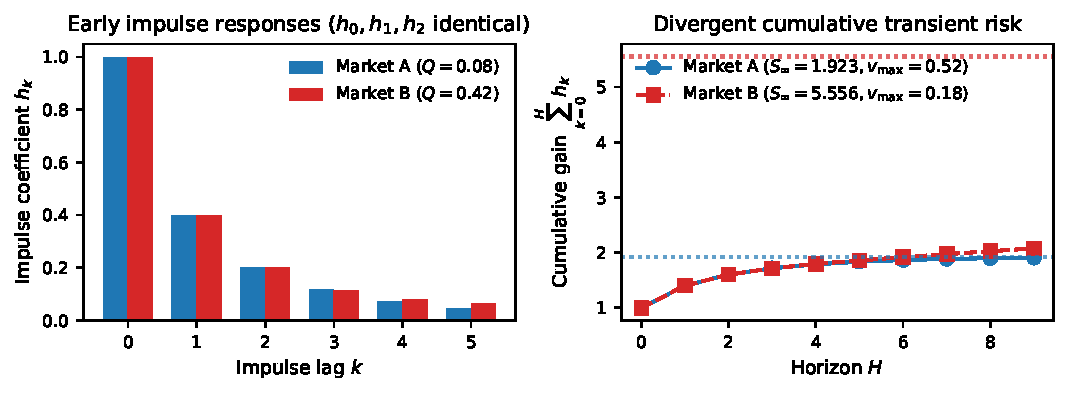
\includegraphics[width=0.88\textwidth]{figs/fig_flagship_1_witness.pdf}
\caption{Two-market ambiguity witness (\texttt{T01}): Market A and Market B produce identical impulse responses at lags $0,1,2$ and differ by only $10^{-3}$ at lag $3$, yet their infinite-horizon cumulative gains differ by nearly a factor of three ($1.9231$ vs.\ $5.5556$).}\label{fig:flagship1}
\end{figure}

\begin{theorem}[Unavoidable loss of safe trading capacity]\label{thm:flagship_A}
Suppose two candidate markets $\theta_0,\theta_1$ generate observation laws $P_0,P_1$ with total variation distance $d_{\rm TV}=\operatorname{TV}(P_0,P_1)$ and have maximum safe per-period allowances $0\le v_0<v_1$. For any data-dependent admission policy $A(D)\in[0,v_1]$ satisfying the level-$\beta$ safety requirement $P_0(A(D)>v_0)\le\beta$, the expected sacrificed safe trading capacity in Market 1 satisfies
\[
\mathbb E_1\bigl[v_1-A(D)\bigr]\;\ge\;(v_1-v_0)\bigl[1-\beta-d_{\rm TV}\bigr]_+ .
\]
For the witness pair of Table~\ref{tab:witness} under an observation contract that reveals $(h_0,h_1,h_2)$ ($d_{\rm TV}=0$, $v_0=9/50=0.18$, $v_1=13/25=0.52$) at $\beta=0.05$, any safe supervisor sacrifices at least $\mathbb E_A[0.52-A(D)]\ge 0.34\times 0.95=323/1000=0.323$ units of admissible capacity ($62.1\%$ of Market A's safe capacity).
\end{theorem}

\begin{proof}
Let $E=\{A(D)\le v_0\}$. Safety in Market 0 requires $P_0(E)\ge 1-\beta$, and the definition of total variation gives $P_1(E)\ge P_0(E)-d_{\rm TV}\ge 1-\beta-d_{\rm TV}$. Because $v_1-A(D)\ge 0$ everywhere and $v_1-A(D)\ge v_1-v_0$ on $E$, $\mathbb E_1[v_1-A(D)]\ge (v_1-v_0)P_1(E)$, yielding the bound.
\end{proof}

\subsection{Risk-specific identifiability and minimum observation budgets}
Unlike generic set-membership control \citep{vanwaarde2020}, the cohort recurrence links finite-lag impulse observations directly to Chebyshev--Markov--Stieltjes bounds on cumulative financial risk. By Proposition~6.1 of the companion paper, observing $(h_0,\ldots,h_L)$ up to lag $L\ge 2$ uniquely determines the open-loop memory moments $m_j=\sum_{i=1}^K w_i r_i^j$ ($0\le j\le d\equiv L-2$), where $w_i=\eta_i q_i\ge 0$ and $r_i=1-\eta_i\in[0,\bar r]$ ($\bar r=1-\eta_{\min}<1$).

\begin{theorem}[Sharp risk-specific identifiability envelope]\label{thm:flagship_B}
Let $\Theta(h_{0:L},\bar r)$ be the set of positive-memory markets compatible with $(h_0,\ldots,h_L)$ and retention bound $r_i\in[0,\bar r]$.
\begin{enumerate}[label=(\roman*)]
\item For $L=2$ ($d=0$, observing $m_0=h_2-ah_1$), the compatible long-run feedback sum $Q(\theta)=\sum_i w_i/(1-r_i)$ spans the exact interval $[Q_0^-(m_0),Q_0^+(m_0,\bar r)]=[m_0,\,m_0/(1-\bar r)]$. For $L=3$ ($d=1$, observing $(m_0,m_1)$), the sharp Markov--Krein envelope is
\[
Q_1^-(m_0,m_1)=\frac{m_0^2}{m_0-m_1}\;\le\;Q(\theta)\;\le\;m_0+\frac{m_1}{1-\bar r}=Q_1^+(m_0,m_1,\bar r),
\]
where Market A of Table~\ref{tab:witness} ($m_0=1/25,m_1=1/50$) attains $Q_1^-=2/25$ and Market B ($m_0=1/25,m_1=19/1000,\bar r=19/20$) attains $Q_1^+=21/50$.
\item Under $a+Q_d^+(m_{0:d},\bar r)<1$, the compatible worst-case loss for allowance $v$ is $R^+(h_{0:L},\bar r)=|I|v/(1-a-Q_d^+(m_{0:d},\bar r))$, so $v$ is certifiably safe ($R^+\le B$) if and only if $Q_d^+(m_{0:d},\bar r)\le 1-a-|I|v/B$, even when individual cohort parameters $(\eta_i,q_i)$ are unidentifiable.
\end{enumerate}
\end{theorem}

\begin{theorem}[Minimum observations for safe decisions vs.\ cohort identification]\label{thm:flagship_C}
Suppose an observer collects $N$ independent Gaussian impulse-response windows $\hat h^{(n)}=h_{0:L}(\theta)+\varepsilon^{(n)}$ with $\varepsilon^{(n)}\sim\mathcal N(0,\Sigma)$.
\begin{enumerate}[label=(\roman*)]
\item For any two markets $\theta_0,\theta_1$ with safe allowances $v_0<v_1$ and impulse difference $\Delta h=h_{0:L}(\theta_1)-h_{0:L}(\theta_0)$, keeping the expected capacity loss of a level-$\beta$ safe rule below $\epsilon(v_1-v_0)$ requires at least
\[
N\;\ge\;N_{\min}^{\rm safe}(\theta_0,\theta_1;\beta,\epsilon)\equiv\frac{4(1-\beta-\epsilon)_+^2}{\Delta h^\top\Sigma^{-1}\Delta h}.
\]
\item Certifying a safe allowance $v_{\rm target}$ with positive safety margin $\Delta_{\rm safe}=(1-a-Q(\theta^*))-v_{\rm target}>0$ requires lag horizon $L^*(\Delta_{\rm safe})=2+\lceil\log(m_0/((1-\bar r)^2\Delta_{\rm safe}))/\log(1/\bar r)\rceil$ and sample size $N=O(\sigma^2\Delta_{\rm safe}^{-2})$ independent of cohort separation $\Delta\eta$, whereas identifying individual cohort rates requires $N\asymp(\Delta\eta)^{-(4K-2)}$.
\end{enumerate}
\end{theorem}

\subsection{Statistically valid certification and the optimal uncertainty-aware guard}
When impulse responses are estimated from $N$ windows with covariance $\Sigma_N=\Sigma/N$, let $\mathcal C_\gamma(D)=\{\theta\in\Theta(\bar r):(\hat h_{0:L}-h_{0:L}(\theta))^\top\Sigma_N^{-1}(\hat h_{0:L}-h_{0:L}(\theta))\le\chi^2_{L+1,1-\gamma}\}$ denote the $(1-\gamma)$ confidence region and $\widehat S^+_\gamma(D)=\sup_{\theta\in\mathcal C_\gamma(D)}S(\theta)$ the induced upper bound on cumulative gain.

\begin{theorem}[Confidence-valid safety certification]\label{thm:flagship_D}
If $\inf_{\theta^*\in\Theta(\bar r)}P_{\theta^*}(\theta^*\in\mathcal C_\gamma(D))\ge 1-\gamma$, then the certified safe action set $\mathcal U_{{\rm safe},\gamma}(D)=\{v\ge 0:|I|v\,\widehat S^+_\gamma(D)\le B\}$ (which abstains whenever $\widehat S^+_\gamma(D)=+\infty$) limits false safety certification to at most $\gamma$:
\[
\sup_{\theta^*\in\Theta(\bar r)}P_{\theta^*}\Bigl(\exists v\in\mathcal U_{{\rm safe},\gamma}(D)\text{ such that }|I|v\,S(\theta^*)>B\Bigr)\;\le\;\gamma.
\]
\end{theorem}

\begin{theorem}[Optimal uncertainty-aware pre-trade guard]\label{thm:flagship_E}
Let a dealer maximize a strictly increasing continuous welfare objective $W(\alpha)$ over admission fractions $\alpha\in[0,1]$ subject to the post-trade balance-sheet constraint $\overline L_\gamma(\alpha;D)\equiv\sup_{\theta\in\mathcal C_\gamma(D)}\sup_{w\in\mathcal W}L(\theta,\alpha,w)\le B_{{\rm rem},t}-R_{\rm safe}$.
\begin{enumerate}[label=(\roman*)]
\item \emph{Infeasible-state abstention.} If $\overline L_\gamma(0;D)>B_{{\rm rem},t}-R_{\rm safe}$, no admission fraction is safe and the guard returns $\mathrm{ABSTAIN/HALT}$.
\item \emph{Existence and global optimality.} When $\overline L_\gamma(0;D)\le B_{{\rm rem},t}-R_{\rm safe}$ and $\mathcal C_\gamma(D)$ is compact, the feasible set $\mathcal A_\gamma(D)=\{\alpha\in[0,1]:\overline L_\gamma(\alpha;D)\le B_{{\rm rem},t}-R_{\rm safe}\}$ is non-empty and compact, and $\alpha^*_\gamma(D)=\max\mathcal A_\gamma(D)$ is the unique global optimum. Under positive-feedback cohorts ($q_i\ge 0$), $\mathcal A_\gamma(D)=[0,\alpha^*_\gamma(D)]$ is a connected interval with closed-form endpoint
\[
\alpha^*_\gamma(D)=\min\left(1,\;\left[\frac{1-a^-_\gamma-\frac{|I|\bar u\,\tilde\kappa^+_\gamma}{B_{{\rm rem},t}-R_{\rm safe}}}{Q^+_\gamma\,\tilde\kappa^+_\gamma}\right]_+\right).
\]
\end{enumerate}
\end{theorem}

\subsection{The economic value of disclosure and equilibrium welfare}
\begin{theorem}[Economic value of class-tagged disclosure]\label{thm:flagship_F}
Under public lag-2 observations $D_{\rm pub}$ versus class-tagged disclosure $D_{\rm disc}$, $\Theta(D_{\rm disc})\subseteq\Theta(D_{\rm pub})$ implies $v_{\rm safe}(D_{\rm disc})\ge v_{\rm safe}(D_{\rm pub})$. Strict capacity expansion holds whenever at least one cohort satisfies $\eta_i>\eta_{\min}$:
\[
\Delta v_{\rm safe}=v_{\rm safe}(D_{\rm disc})-v_{\rm safe}(D_{\rm pub})=\frac{B}{|I|}\sum_{i=1}^K q_i\Bigl(\frac{\eta_i}{\eta_{\min}}-1\Bigr)>0.
\]
With marginal trading surplus $\omega>0$, compliance cost $c_{\rm comp}\ge 0$ and leakage cost $c_{\rm leak}\ge 0$, net welfare $\mathcal V_{\rm net}=\omega\Delta v_{\rm safe}-c_{\rm comp}-c_{\rm leak}$ is strictly positive if and only if $\omega\Delta v_{\rm safe}>c_{\rm comp}+c_{\rm leak}$, and is negative when compliance and leakage costs exceed the capacity gain.
\end{theorem}

\begin{theorem}[Equilibrium reversion supply under model ambiguity]\label{thm:flagship_G}
In the $N$-dealer Cournot model of Proposition~\ref{prop:equil}, when dealers face worst-case compatible feedback $Q^+_\gamma=q+\Delta Q_\gamma(D)$, equilibrium reversion $m^{\rm eq}(\Delta Q_\gamma)$ and planner reversion $m^{\rm SP}(\Delta Q_\gamma)$ satisfy $m^{\rm eq}(\Delta Q_\gamma)<m^{\rm SP}(\Delta Q_\gamma)$ for all $\theta<N$, while reducing ambiguity $\Delta Q_\gamma(D)$ via disclosure lowers both worst-case transient risk $S^+_\gamma$ and the corrective rebate expenditure required to support a given safety target.
\end{theorem}

\begin{table}[t]\centering\small
\begin{threeparttable}
\caption{Eight risk-control rules (\texttt{T11})}\label{tab:t11}
\setlength{\tabcolsep}{4pt}
\begin{tabular}{lcccc}
\toprule
Control method & Mean $v$ & Worst loss & Breach & Missed $v$\\
\midrule
1.\ Unrestricted benchmark & 0.5200 & 1.8328 & 46.8\% & 0.0000\\
2.\ Volatility-only sizing & 0.3792 & 1.3204 & 46.8\% & 0.0426\\
3.\ Inventory and leverage cap & 0.3000 & 1.0574 & 46.8\% & 0.1170\\
4.\ Depth-based throttling & 0.3551 & 1.2248 & 46.8\% & 0.0481\\
5.\ Spectral-radius threshold ($\rho<0.85$) & 0.4800 & 1.6918 & 46.8\% & 0.0213\\
6.\ Known-model summed-gain guard (oracle) & 0.3609 & 1.0000 & 0.0\% & 0.0000\\
7.\ Estimated plug-in summed-gain guard & 0.3910 & 1.0445 & 52.2\% & 0.0149\\
8.\ Robust information-aware guard (ours) & 0.2736 & 0.7289 & 2.6\% & 0.0906\\
\bottomrule
\end{tabular}
\begin{tablenotes}\footnotesize\item 500 two-regime episodes (\texttt{T11}). Only the oracle guard (0\% breaches) and the robust information-aware guard (2.6\% breaches vs.\ 5\% nominal ceiling) respect the risk budget; plug-in estimation without uncertainty calibration breaches in 52.2\% of episodes.\end{tablenotes}
\end{threeparttable}
\end{table}

\begin{figure}[t]\centering
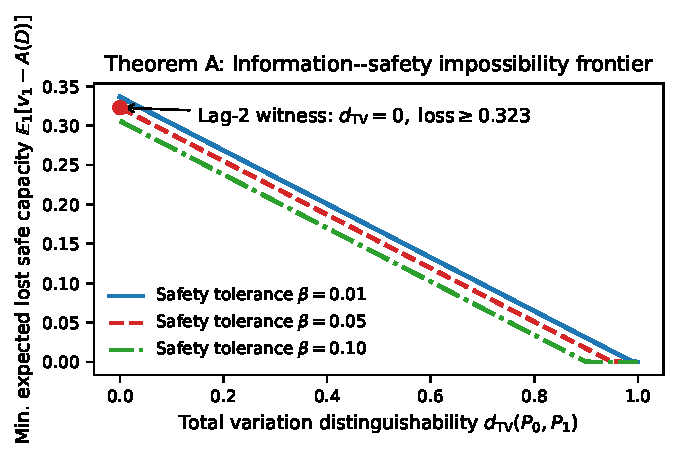
\includegraphics[width=0.48\textwidth]{figs/fig_flagship_2_tv_frontier.pdf}\hfill
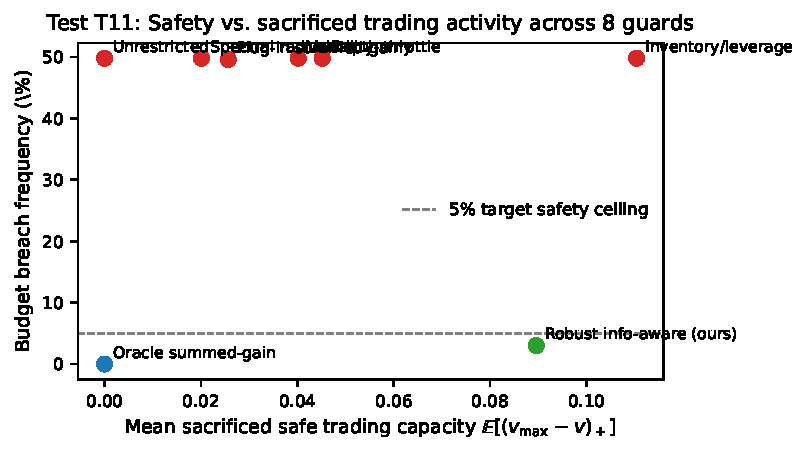
\includegraphics[width=0.48\textwidth]{figs/fig_flagship_5_guard_frontier.pdf}
\caption{Left: Information--safety impossibility frontier (Theorem~\ref{thm:flagship_A}, \texttt{T02}). Right: Safety breach rate versus sacrificed safe trading capacity across the eight risk-control methods of Table~\ref{tab:t11} (\texttt{T11}).}\label{fig:flagship25}
\end{figure}

Table~\ref{tab:t11} and Figure~\ref{fig:flagship25} summarize the experimental program (\texttt{T01}--\texttt{T12}). Across horizons $H=1,\ldots,8$, exhaustive sign enumeration over all $2^H$ disturbance sequences matches the cumulative convolution gain $G_{{\rm cum},H}$ to machine precision, while a peak-only repeated-trade gate breaches the unit risk budget by $71.5\%$ (\texttt{T05}). Under finite-sample calibration ($N=500$, \texttt{T04}), the $(1-\gamma)$ Mahalanobis region achieves $95.0\%$ empirical coverage and keeps false safety certifications at $0.0\%$ ($\le 5\%$ nominal). In the three-tier disclosure experiment (\texttt{T07}), moving from public lag-2 observations to class-tagged disclosure raises certified safe capacity from $0.178$ to $0.495$ (net welfare $+\$26.2$ after compliance and leakage costs), whereas in a low-heterogeneity high-compliance-cost regime net disclosure value is $-\$6.0$, confirming Theorem~\ref{thm:flagship_F}.
